\section{Mutation}\label{mutation}

Unter der Mutation versteht man die zufällige Veränderung einiger Gene eines
Individuums.
Bei dem \emph{Travelling Salesman Problem} mit der Pfad-Darstellung
können bei willkürlicher Modifikation natürlich ungültige Chromosome
entstehen.
Die folgenden drei verwendeten Verfahren vermeiden allerdings die Erzeugung
ungültiger Chromosome, da sie nur die Positionen der Gene innerhalb des
Chromosoms verändern.

% http://www.geatbx.com/docu/options-04.html

\subsection{mutmove}
Bei allen hier beschriebenen Mutationsverfahren werden zufällig zwei Positionen
innerhalb des Chromosoms ausgewählt (in Abbildung \ref{fig.mutation} mit den
roten Pfeilen dargestellt).
Bei \emph{mutmove} wird das Element bei der hinteren Position herausgenommen und
an der vorderen Position wieder eingefügt, wobei die Elemente zwischen den zwei
gewählten Positionen jeweils um eine Position aufrücken \citep{mutation}.

\begin{figure}[h!]
  \centering
  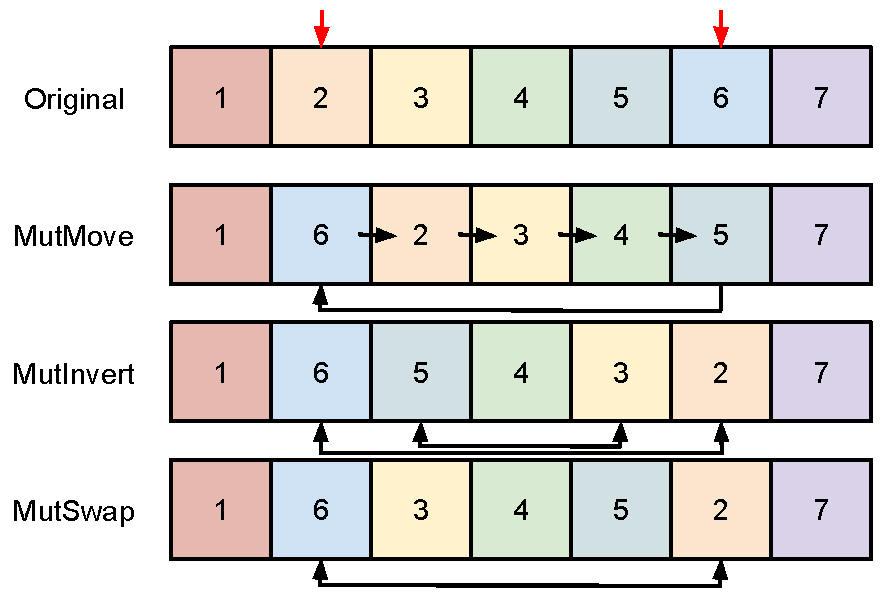
\includegraphics[width=0.7\textwidth]{Figures/mutation.pdf}
  \caption{Mutationsverfahren}\label{fig.mutation}
\end{figure}


\subsection{mutinvert}
Die beiden gewählten Positionen innerhalb des Chromosoms beschreiben Anfang
und Ende eines Substrings, welcher aus dem Chromosom entnommen und danach
mit invertierter Reihenfolge der Elemente wieder an der gleichen Position
eingefügt wird.
Die entstehende Reihenfolge im Chromosom ist ebenfalls beispielhaft in Abbildung
\ref{fig.mutation} dargestellt \citep{mutation}.


\subsection{Ergebnisse}

Die beiden bisher genannten Verfahren werden mit dem \emph{mutswap}
Verfahren aus \citep{erben} verglichen, bei dem die beiden Elemente an den zwei
Positionen einfach vertauscht werden.
Für die Mutations-Testläufe wurde die Mutationsrate jeweils bei allen 3 verschiedenen
Verfahren verändert.
Die folgenden Zeilen Quelltext enthalten die entsprechenden Aufrufe von
{\tt testTsp()}:

\lstinputlisting[language=MATLAB, firstline=44, lastline=51]{Code/suite.m}

\input{Chapters/gen/Mutation.Rate.mutmove}

\input{Chapters/gen/Mutation.Rate.mutinvert}

\input{Chapters/gen/Mutation.Rate.mutswap}

\begin{figure}[!h]
\minipage{0.32\textwidth}
  \includegraphics[width=\linewidth]{Figures/gen/Mutation.Rate.mutmove.png}
  \caption{mutmove}\label{fig:mutmove}
\endminipage\hfill
\minipage{0.32\textwidth}
  \includegraphics[width=\linewidth]{Figures/gen/Mutation.Rate.mutinvert.png}
  \caption{mutinvert}\label{fig:mutinvert}
\endminipage\hfill
\minipage{0.32\textwidth}%
  \includegraphics[width=\linewidth]{Figures/gen/Mutation.Rate.mutswap.png}
  \caption{mutswap}\label{fig:mutswap}
\endminipage
\end{figure}

Alle Verfahren performen ähnlich gut (vergleiche Abbildungen
\ref{fig:mutmove} bis \ref{fig:mutswap}), daher fällt es schwer eine eindeutige
Auswahl zu treffen.
Für die optimale Parameterkonfiguration entscheiden wir uns für
{\tt mutmove} mit einer Mutationsrate von 1,25 Mutationen pro Individuum.

